\documentclass{article}
\usepackage[T1]{fontenc}
\usepackage[preprint]{neurips_2026}
\usepackage{amsmath,amssymb,booktabs,placeins,graphicx}
\usepackage[hidelinks]{hyperref}

\title{Concurrent Subspaces Analysis:\\
A Critical Study and Experimental Reproduction}
\author{Ding Yuanwei, Guan Tik Sha, Ng Cheuk Tung, and Wang Zhengwei\\
COMP3314 Group 22, The University of Hong Kong}

\begin{document}
\maketitle
\begin{abstract}
Concurrent Subspaces Analysis (CSA) learns compact tensor representations through
coupled orthogonal projections. We explain its reconstruction objective and exact
alternating updates, relate it to PCA, LDA, and nearest-neighbor recognition, and
evaluate the evidence in the original paper. Our independent reproduction on
ORL, MNIST, and grayscale FERET supports substantial projection-storage savings
but conditional recognition gains. Controlled comparisons reveal sensitivity to
feature dimensions, preprocessing, and distance metrics. We distinguish
optimization guarantees from generalization claims and identify validation
priorities for further work.
\end{abstract}

\section{Problem and Contributions}
\label{sec:overview}
\subsection{Task and motivation}
\citet{xu2008csa} study how to compress tensor-valued objects while retaining
information for reconstruction and recognition. Vectorized image features can
be high-dimensional relative to the training set: their ORL recognition setting
uses $28\times23\times40=25{,}760$ Gabor values per image but only two training
images per identity, or 80 in total. The challenge is to learn a useful compact
representation from limited data, not simply to reshape the input.

\subsection{Central idea and contributions}
CSA learns shared bases along each object's modes and a small core for each
sample. Its contributions are a reconstruction criterion for arbitrary-order
tensors, an alternating eigendecomposition algorithm, a constrained-PCA
interpretation, and reconstruction/recognition experiments on faces and digits.
Unlike Tensorface's organization of an image ensemble by identity, pose, and
illumination, CSA's axes describe an individual object, such as height, width,
and filter channel \citep[Sec.~III-A]{xu2008csa}. This distinction makes axis
definition a modeling choice, rather than treating all tensor representations
as interchangeable.

\section{Methods}
\label{sec:methods}
\subsection{Representation and reconstruction objective}
For $N$ tensors $\mathcal X_i\in\mathbb R^{m_1\times\cdots\times m_K}$,
choose dimensions $r_k\leq m_k$ and shared bases
$U_k\in\mathbb R^{m_k\times r_k}$ with $U_k^\top U_k=I$.
CSA encodes and reconstructs each sample as
\begin{equation}
\mathcal Y_i=\mathcal X_i\times_1U_1^\top\cdots\times_KU_K^\top,
\qquad \widehat{\mathcal X}_i=\mathcal Y_i\times_1U_1\cdots\times_KU_K,
\label{eq:encoding}
\end{equation}
where $\times_k$ multiplies along mode $k$. The bases minimize
$E=\sum_i\|\mathcal X_i-\widehat{\mathcal X}_i\|_F^2$.
Orthogonal projection gives
$E=E_0-\sum_i\|\mathcal Y_i\|_F^2$, with constant
$E_0=\sum_i\|\mathcal X_i\|_F^2$; minimizing reconstruction error therefore
maximizes retained core energy \citep[Sec.~II-B]{xu2008csa}.

\subsection{Alternating optimization}
Initialize column-orthonormal bases. Fix all modes except $k$, project along
those fixed modes, and unfold each result into
$B_i^{(k)}\in\mathbb R^{m_k\times\prod_{j\ne k}r_j}$.
The core unfolding is $U_k^\top B_i^{(k)}$, so
\begin{equation}
C_k=\sum_iB_i^{(k)}B_i^{(k)\top},\qquad
E(U_k\mid U_{-k})=E_0-\operatorname{tr}(U_k^\top C_kU_k).
\label{eq:conditional}
\end{equation}
Here $U_{-k}$ denotes the fixed bases. The leading $r_k$ eigenvectors of $C_k$ maximize the trace
\citep[Theorem~1]{xu2008csa}. With eigenvalues in descending order,
\begin{equation}
E_{\mathrm{new}}-E_{\mathrm{old}}
=\operatorname{tr}\!\bigl((U_k^{\mathrm{old}})^\top C_kU_k^{\mathrm{old}}\bigr)
-\sum_{j=1}^{r_k}\lambda_j(C_k)\leq0.
\label{eq:nonincrease}
\end{equation}
The old basis remains feasible for the same conditional problem, so its exact
optimum cannot be worse. Cycle through the modes using the latest bases until
stabilization or an iteration limit. These updates are coupled through $C_k$.
At fixed ranks and preprocessing, the nonnegative objective is non-increasing
and converges; this proves neither global optimality nor convergence of the
bases. Appendix~\ref{app:proof} supplies the detailed argument.

\subsection{Course connections and recognition}
With consistent column-major vectorization,
$\operatorname{vec}(\mathcal Y_i)=P^\top\operatorname{vec}(\mathcal X_i)$ for
$P=U_K\otimes\cdots\otimes U_1$.
CSA constrains the PCA-like projection to a Kronecker structure; flattening
itself is lossless. The eigenupdate connects to PCA: for centered inputs,
maximizing retained energy maximizes variance; otherwise it uses second moments
\citep[Sec.~III-B]{xu2008csa}. For recognition, vectorize the core, optionally apply Fisher
LDA, and classify by 1-NN \citep[Sec.~IV-C]{xu2008csa}.
LDA uses labels to favor between-class over within-class scatter,
while 1-NN assigns the closest gallery label. These connect CSA's recognition
pipeline to supervised dimensionality reduction and instance-based learning
covered in the course.
CSA itself is unsupervised, so improved reconstruction need not improve recognition.

\section{Evidence and Reproduction}
\label{sec:evidence}
\subsection{What the original paper establishes}
\label{sec:csa-paper-evidence}
The paper evaluates reconstruction on ORL and CMU PIE and recognition on ORL,
CMU PIE, FERET, and MNIST. For reconstruction, one image per identity is used;
the compression ratio counts both shared projection matrices and per-image
coefficients. The paper's Figure~5 reports lower reconstruction RMSE for CSA at comparable
storage budgets. Its Figure~4 shows near-stable projections by approximately three
iterations in the illustrated ORL run, an empirical observation rather than a
universal bound. Recognition uses 1-NN with optional LDA, including ORL's
two-gallery/eight-probe split and FERET's disjoint training/test identities.
Table~\ref{tab:recognition} reproduces selected paper results: for Gabor ORL,
direct CSA reaches 94.40\% with 390 coefficients versus PCA's 86.60\% with 76.
These support the reported configurations; they do not isolate representation
quality at equal output dimension. The authors report best parameter settings,
with repeated-split aggregation unspecified \citep[Sec.~IV]{xu2008csa}.

\subsection{Our implementation and scope}
We independently implemented CSA, PCA, Fisher LDA, and evaluation code using
NumPy/SciPy for numerical operations and Pillow/OpenCV for image processing;
YuNet detection assets are reused. We reproduced ORL, MNIST, and original
grayscale FERET experiments; CMU PIE was unavailable and omitted with instructor
permission. Code, run instructions, provenance, and recorded results are at
\url{https://github.com/gwdsd1/COMP3314GP}.

ORL uses ten splits with two gallery and eight probe images per identity;
MNIST uses three splits with 30 or 40 training images per digit; FERET uses one
fixed identity partition for each training size. Methods share input arrays,
splits, and distance within each comparison: Euclidean for current ORL and
cosine for MNIST/FERET. Recognition PCA is centered and CSA uncentered, so this
does not isolate the projection constraint under identical centering.
ORL preprocessing retains earlier probe-informed exploration, including the
Gabor context extension. These scores are not fresh blind-test estimates.
Appendix~\ref{app:protocol} details input conventions and deviations from the paper.

\subsection{Results and controlled comparisons}
\begin{table}[!ht]
\centering
\small
\setlength{\tabcolsep}{4pt}
\caption{Top-1 accuracy (\%). Paper columns are from \citet{xu2008csa},
Tables I, II, and IV; ours are recorded group experiments, not new runs for this
report. ORL/MNIST show mean $\pm$ sample SD over ten/three splits; FERET uses
one partition per training size. Dimensions follow each paper configuration.}
\label{tab:recognition}
\begin{tabular}{@{}lrrrr@{}}
\toprule
&\multicolumn{2}{c}{PCA}&\multicolumn{2}{c}{CSA}\\
\cmidrule(lr){2-3}\cmidrule(l){4-5}
Setting&Paper&Ours&Paper&Ours\\
\midrule
ORL gray + LDA&82.20&$77.22\pm2.35$&84.10&$81.72\pm2.06$\\
ORL Gabor, direct NN&86.60&$86.91\pm1.60$&94.40&$89.66\pm1.92$\\
ORL Gabor + LDA&87.20&$88.41\pm1.96$&90.90&$87.53\pm2.91$\\
MNIST, 30 train/class&88.50&$87.52\pm0.40$&92.80&$90.34\pm0.15$\\
MNIST, 40 train/class&90.50&$88.58\pm0.37$&92.40&$91.04\pm0.25$\\
FERET, 50 train identities&84.60&89.08&88.20&88.73\\
FERET, 100 train identities&90.60&90.87&92.20&94.25\\
FERET, 200 train identities&93.40&93.87&95.20&95.38\\
\bottomrule
\end{tabular}
\end{table}
\FloatBarrier

CSA exceeds our PCA baseline in six of eight configurations. MNIST preserves
the paper's CSA-over-PCA ordering; FERET CSA matches or exceeds its reported
values, but loses to our PCA at 50 training identities. All three ORL CSA means
remain below the paper. Our ORL reconstruction and projection-stabilization
records recover the qualitative trends (Appendix~\ref{app:reconstruction}),
rather than exact author-identical curves.

The Gabor LDA row compares CSA $24\to23$ with PCA $33\to25$.
Matching both at $24\to23$ yields 87.53\% versus 85.72\% under Euclidean distance,
a CSA advantage of 1.81 percentage points. Applying centered cosine to the same
fitted models instead gives 88.75\% versus 90.59\%, reversing the ordering.
Figure~\ref{fig:metric} shows that recognition gains depend on the metric, even
with fixed representations.
In a separate 20-split centered-cosine control at Gabor $\sigma=\pi$, extending filtering beyond
the crop raises CSA from 81.25\% to 87.08\%, while matched context PCA reaches
91.08\%. Better preprocessing therefore need not establish a CSA advantage.

\begin{figure}[!ht]
\centering
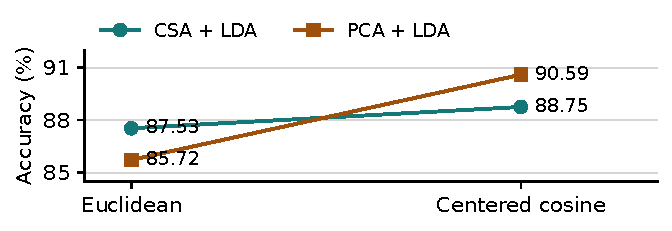
\includegraphics[width=0.78\linewidth]{figures/metric_comparison.pdf}
\caption{Our matched-dimension ORL Gabor results: ten-split means for
CSA and PCA, both $24\to23$. Only the distance rule changes between columns;
the fitted models and splits are fixed. Source: group records listed in
Appendix~\ref{app:controls}.}
\label{fig:metric}
\end{figure}
\FloatBarrier

\clearpage
\section{Critical Analysis and Team Insights}
\label{sec:analysis}
\subsection{Structural bias, sample size, and computational cost}
CSA assumes that objects share useful mode-specific linear subspaces. Aligned
axes make this plausible for the studied images, but a single Kronecker product
restricts which joint subspaces can be represented. Separate mode matrices do
not imply statistically independent variation. Shorter unfolded fibers give
smaller estimation problems, yet fibers from one image are correlated, not new
independent training images. Compact structure may improve generalization with
scarce data, but the fiber count alone cannot guarantee it.

The clearest benefit is projection storage: CSA needs $\sum_km_kr_k$ entries,
versus $Dd$ for dense PCA, where $D=\prod_km_k$ and $d=\prod_kr_k$.
For Gabor $28\times23\times40\to4\times2\times3$, including an LDA map of the same
$24\to23$ size gives 830 versus 618,792 weights. This is not a peak-memory or universal
runtime claim. Sample-space PCA can use an $N\times N$ eigenproblem
when $N\ll D$ \citep[p.~40, footnote~2]{xu2008csa}; CSA also pays for tensor contractions and
repeated updates.

\subsection{What constitutes convincing evidence}
At equal output dimension and identical centered inputs, unrestricted PCA has
no higher optimal training reconstruction error than its constrained counterpart.
CSA's equal-storage advantage is compatible with this: cheaper shared bases
leave more budget for core coefficients. The budget, not simply the algorithm
name, determines which claim is being tested.

Recognition is a different objective. High-energy lighting variation may be
uninformative about identity, and LDA is not an automatic remedy. The paper's
90.90\% for CSA+LDA is below direct CSA's 94.40\% on ORL; the authors suggest
overfitting \citep[Sec.~IV-C]{xu2008csa}, but their different core dimensions prevent attributing the entire
gap to LDA. Likewise, our metric reversal demonstrates pipeline dependence.
Cross-paper differences are descriptive: the paper's split aggregation is
unspecified, preprocessing and partitions may differ, historical probes
influenced development, and repeated splits reuse images. FERET agreement therefore does not prove a
better implementation or statistically significant superiority.

\subsection{Lessons and targeted improvements}
Our central lesson is to separate three questions: what structure is imposed,
what the optimizer guarantees, and what the evaluation measures. Vectorization
preserves values; CSA's restriction on the projection changes the hypothesis
class. Exact conditional minimization explains stable reconstruction error,
but does not establish a globally best representation or a better classifier.

Future evaluation should freeze preprocessing and metrics, select ranks within
training-only validation, compare both equal-dimension and equal-storage
budgets, and use fresh held-out data. Multiple orthogonal starts can measure
initialization sensitivity, without claiming global optimality. Regularized LDA
or supervised tensor objectives can target discrimination, but our negative
DATER experiment (Appendix~\ref{app:controls}) shows that adding labels alone
is insufficient evidence of improvement. More flexible or nonlinear representations
are possible extensions, with additional capacity and validation costs; they are
not automatic solutions to the Kronecker restriction. Overall, CSA offers a
compact, interpretable structural bias whose recognition benefits remain
conditional on the data and evaluation protocol.

\label{end:main}

\clearpage
\bibliographystyle{plainnat}
\bibliography{references}
\clearpage
\appendix
\section{Details of the Optimization Argument}
\label{app:proof}
\subsection{Orthogonal projection and retained energy}
Let $x_i=\operatorname{vec}(\mathcal X_i)$ and
$P=U_K\otimes\cdots\otimes U_1$. The Kronecker product identities give
$P^\top P=(U_K^\top U_K)\otimes\cdots\otimes(U_1^\top U_1)=I$.
Thus $Q=PP^\top$ is symmetric and idempotent, so
\begin{equation}
\|x_i-Qx_i\|_2^2
=x_i^\top(I-Q)^2x_i
=\|x_i\|_2^2-x_i^\top Qx_i
=\|x_i\|_2^2-\|P^\top x_i\|_2^2.
\end{equation}
Since $P^\top x_i=\operatorname{vec}(\mathcal Y_i)$, summation yields the energy
identity in Section~\ref{sec:methods}. This identity holds without centering;
centering is needed for the usual variance interpretation.

\subsection{Why the eigenvector update is optimal}
For three-mode tensors, fixing $U_2,U_3$ gives
$B_i=(\mathcal X_i\times_2U_2^\top\times_3U_3^\top)_{(1)}$.
Both $B_i$ and $C_1=\sum_iB_iB_i^\top$ stay fixed while optimizing $U_1$.
Because unfolding preserves the Frobenius norm,
$\sum_i\|U_1^\top B_i\|_F^2=\operatorname{tr}(U_1^\top C_1U_1)$.
The same argument applies to every mode.

Write $C_k=V\Lambda V^\top$, with orthonormal eigenvectors $v_j$ and descending
eigenvalues $\lambda_j$. Any feasible $U$ satisfies
\begin{equation}
\operatorname{tr}(U^\top C_kU)=\sum_j\lambda_jw_j,
\quad w_j=\|v_j^\top U\|_2^2\in[0,1],
\quad\sum_jw_j=r_k.
\end{equation}
The bounds follow because $UU^\top$ is a rank-$r_k$ orthogonal projector.
The weighted sum is at most $\sum_{j=1}^{r_k}\lambda_j$, attained by
$U=[v_1,\ldots,v_{r_k}]$. Since the old basis is feasible, this proves
Equation~\eqref{eq:nonincrease}, expanding Theorem~1 of \citet{xu2008csa}.
Successive exact updates satisfy
$E^{(t,0)}\geq E^{(t,1)}\geq\cdots\geq E^{(t,K)}=E^{(t+1,0)}\geq0$.
Ranks, data, and preprocessing remain fixed. Equality and nonunique bases can
occur, especially with repeated eigenvalues; objective convergence does not
prove convergence of the bases or a strict local minimum. Numerical checks
must allow floating-point tolerance.

\section{Reproduction Protocols and Supplementary Evidence}
\label{app:protocol}
\subsection{Inputs, splits, and implementation choices}
ORL contains 400 images from 40 identities \citep{orlData}. Recognition uses
aligned/equalized $56\times46$ grayscale images or $28\times23\times40$ Gabor
magnitudes. The current comparison uses seeds 20--29, shared inputs and
Euclidean 1-NN, with unit-length LDA columns. CSA runs at most three sweeps;
CSA24 uses HOSVD initialization, while grayscale/direct CSA390 use rectangular
identity bases. The $\pi$-context Gabor input filters an expanded aligned image
before extracting the central response. It is a declared extension, not an
author-confirmed preprocessing choice. All current ORL inputs retain previous
probe-informed development; the final fixed batch performs no new search but
is not an independent blind test.

For the metric comparison, the gallery feature mean is subtracted from both
gallery and probe embeddings before scoring. This common translation leaves
Euclidean distances unchanged but defines the centered-cosine rule. The fitted
CSA/PCA/LDA maps remain fixed; this scoring step is distinct from centering
the training inputs when fitting PCA.

MNIST uses the first 500 images of each digit in the official test set,
5,000 images total \citep{lecun1998mnist}, with $28\times28\times40$ Gabor features.
Each split selects 30 or 40 training examples per class, leaving 470 or 460
probes. The original paper describes the ``first half'' of the test set and
also 500 images per class; our balanced selection is explicit, but the authors'
exact indices are unavailable. The recognition dimensions are listed in
Table~\ref{tab:configurations}; the distance is cosine.

We use original grayscale FERET \citep{phillips2000feret}, with 1,195 Fa/Fb
identity pairs as in \citet[Sec.~IV-A]{xu2008csa}, aligned/equalized to $41\times27$.
For $q=50,100,200$, the first $q$ paired identities provide training Fa+Fb;
remaining Fa images form the gallery and Fb images the probes. The table uses
fixed cosine controls, not validation-selected winners.
Identity ordering and precise alignment conventions are not confirmed identical
to the paper. Recognition PCA is centered and CSA uncentered in all three datasets.

The group implements the learning and evaluation algorithms; scientific
libraries, BLAS/LAPACK, image utilities, and pretrained detectors are reused
components. The repository documents dependencies, data acquisition, model
settings, source attribution, and verification. Raw datasets and feature/model
caches are not distributed; regenerating full checks requires the data and
documented preparation stages. This report audits saved records and does not
claim a fresh end-to-end rerun.

\subsection{Exact recognition configurations}
\begin{table}[!ht]
\centering
\small
\setlength{\tabcolsep}{4pt}
\caption{Recorded group configurations for the eight comparisons in
Table~\ref{tab:recognition}. An arrow gives the output dimension after LDA;
no arrow means direct 1-NN. The CSA tuple lists mode ranks, not only their
product. $G$ is training images per digit and $q$ is training identities.
These recognition runs use centered PCA and uncentered CSA.}
\label{tab:configurations}
\begin{tabular}{@{}llllr@{}}
\toprule
Setting & PCA $\to$ LDA & CSA ranks $\to$ LDA & Distance & Splits\\
\midrule
ORL gray & $30\to18$ & $11\times2\to16$ & Euclidean & 10\\
ORL Gabor, direct & $76$ & $15\times1\times26$ & Euclidean & 10\\
ORL Gabor + LDA & $33\to25$ & $4\times2\times3\to23$ & Euclidean & 10\\
MNIST, $G=30$ & $60$ & $5\times9\times18$ & Cosine & 3\\
MNIST, $G=40$ & $50$ & $15\times5\times13$ & Cosine & 3\\
FERET, $q=50$ & $45\to25$ & $10\times4\to35$ & Cosine & 1\\
FERET, $q=100$ & $95\to40$ & $11\times5\to44$ & Cosine & 1\\
FERET, $q=200$ & $112\to69$ & $13\times7\to62$ & Cosine & 1\\
\bottomrule
\end{tabular}
\end{table}
\FloatBarrier
For the matched-dimension control in Figure~\ref{fig:metric}, PCA changes to
$24\to23$, while CSA remains $4\times2\times3\to23$.
Changing the distance does not refit these models. The table records the
implemented rank allocation; unavailable author code and input settings
prevent a claim of completely author-identical pipelines.

\subsection{Controlled extensions and traceable records}
\label{app:controls}
The 20-split $\sigma=\pi$ crop/context comparison uses centered cosine and fixed
$24\to23$ dimensions. Filtering beyond the crop changes the effective field of
view, so its benefit cannot be attributed solely to the learned representation.
With five probes held fixed per ORL identity, increasing the gallery from two
to three to five gives CSA+LDA 81.30\%, 88.10\%, and 94.50\%; both the fitting
data and reference coverage change.
Our supervised DATER extension \citep{yan2005dater} reaches
$67.11\pm3.59$\% after LDA versus matched CSA's $80.13\pm3.49$\% in the crop-only
control. However, 19 of 20 DATER runs hit the 20-iteration cap, so this is a
negative result for the tested implementation/configuration, not evidence that
supervised tensor methods generally fail.

{\raggedright
The main table is traceable to
\path{results/orl_euclidean_20261104/comparison.csv} and the MNIST/FERET records in
\path{results/orl_protocol_audit/shared_comparison.csv}.
Metric comparisons use \path{results/orl_euclidean_20261104/paired_comparisons.csv};
input controls and weight counts use \path{results/orl_controlled/summary.csv}
and \path{results/orl_controlled/cost_benchmark.csv}.
The gallery-size and DATER sources are \path{results/orl_sample_size/summary.json}
and \path{results/orl_dater/summary.csv}. Qualitative reconstruction and
convergence are recorded in \path{results/available_reproduction_v2/orl_reconstruction.csv}
and \path{results/available_reproduction_v2/orl_convergence.json}.
These are group results; all paper values in Table~\ref{tab:recognition}
are separately attributed to \citet{xu2008csa}.\par}

\clearpage
\section{Recorded Reconstruction and Convergence Diagnostics}
\label{app:reconstruction}
\subsection{Diagnostic setup and comparison budget}
Figure~\ref{fig:reconstruction} uses our saved historical ORL reconstruction
batch: one image per identity (\path{s*/1.pgm}), $N=40$, with full-resolution
$56\times46\times40$ Gabor tensors, $D=103{,}040$ values per object.
Both PCA and CSA are uncentered, and error is evaluated on those same fitting
images. These inputs use historical Haar-based eye alignment with 16 approximate
visual corrections and $\sigma=2\pi$ reflected-boundary filtering. They differ from
the current YuNet/context recognition inputs. Thus the figure illustrates
compression of fitted objects, not unseen-image generalization or the current
recognition protocol.

For stored scalar count $S$, the recorded definitions are
\begin{equation}
\begin{aligned}
\mathrm{CR}&=\frac{ND}{S},&
\mathrm{RMSE}&=\sqrt{\frac{\mathrm{SSE}}{N}},\\
S_{\mathrm{PCA}}&=d(N+D),&
S_{\mathrm{CSA}}&=Nr^3+(56+46+40)r.
\end{aligned}
\end{equation}
The CSA grid uses equal mode ranks $r=1,\ldots,40$; PCA uses $d=1,\ldots,40$.
Each reconstruction CSA fit allows up to ten sweeps with the usual early
stopping rule enabled.
Storage includes cores and bases, with no mean vector for these uncentered
models. RMSE is per object, not per scalar/pixel. The CSV field
\texttt{paper\_rmse} names this definition; its values are our measurements.
The discrete compression grids differ. As a concrete comparison without
interpolation, PCA with $d=2$ stores 206,160 scalars and has RMSE 3458.78;
CSA with $r=17$ stores fewer scalars (198,934) and has RMSE 1624.32.
This supports an advantage at that storage cap, not superiority at equal
coefficient count or across all budgets.

\subsection{Observed convergence and its limits}
The diagnostic uses a $10\times10\times10$ core and rectangular-identity
initialization. Early stopping is disabled to record ten sweeps; recognition
still uses at most three. SSE falls from $2.570566\times10^9$ at initialization
to $2.039869\times10^8$ after one sweep and $2.033656\times10^8$ after three.
Similarity is the average absolute inner product of corresponding old/new
basis columns. All three recorded similarities exceed $0.9999999$ at sweep
three. Later SSE substep increases are at most approximately $3.34\times10^{-6}$,
about $1.64\times10^{-14}$ relative to the loss, consistent with floating-point
effects rather than a strict numerical decrease at every step.
This is an observed trajectory, not proof of global optimality or a universal
three-sweep guarantee.

\begin{figure}[!ht]
\centering
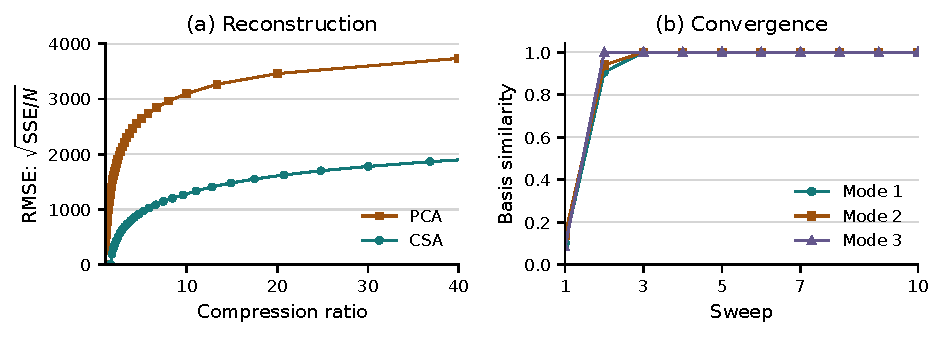
\includegraphics[width=\linewidth]{figures/reconstruction_convergence.pdf}
\caption{Our recorded reconstruction and convergence diagnostics on 40 ORL
fitting images. Left: compression ratio includes basis storage; markers show
recorded settings and connecting lines guide the eye. The displayed range is
restricted to CR $1$--$40$, not the entire CSA grid. Right: successive-basis
similarity for the $10\times10\times10$ diagnostic with early stopping disabled.
These are group records, not digitized paper curves; absolute feature scaling
is not established as author-identical. Sources: the reconstruction and
convergence records listed in Appendix~\ref{app:controls}.}
\label{fig:reconstruction}
\end{figure}
\FloatBarrier

\end{document}
